\chapter{Strategies and Results}
\section{Data Preprocessing}

\subsection{Bucketing}
Before we explain why we need bucketing, we can first explain the structure of our data. When one particle interacts with the detector, it will produce a series of hits, which we call one shower. So in one shower, we have several hits, while one hit means one point in the detector labeled by the energy. One hit has several features, such as the hit energy, x, y and z coordinates. What's more, we will send several showers make it to be one batches to our model. So the structure of our data is actually a 3D tensor, where the first dimension is the number of showers, the second dimension is the number of hits in one shower, and the third dimension is the number of features in one hit.

In chapter 5, we have discussed that our model is a transformer-based model. While transformer implement the self-attention mechanism, it requires the length of the sequence to be fixed in each batches. However, the number of hits in each event varies, which makes it difficult to feed the data into the transformer. To address this issue, we would need to pad the sequences to a fixed length. What's more, the length of the data can vary from 1 to 5500, which means that the padding will be very large. This will lead to a waste of memory and computation. To solve this problem, we employed a bucketing strategy to group events with similar numbers of hits into the same bucket. This allowed us to pad the sequences within each bucket to a fixed length, making it easier to feed the data into the transformer. Based on the principle of similar memory usage, we divided the data into 45 buckets, each containing events with a similar number of hits. This bucketing strategy significantly improved the efficiency of the model and reduced the computational burden. Another advantage of bucketing is that we can first train the model on a smaller bucket to see if the model can learn the data well. If the model can learn the data well, we can then train the model on a larger bucket. This allows us to gradually increase the complexity of the data and ensure that the model can handle the data effectively.
\subsection{Preprocessor}

Preprocessing is a crucial step in preparing data for machine learning. Raw data often contains missing values, outliers, and features on different scales, which can negatively impact model performance. Effective preprocessing cleans and standardizes the data, ensuring consistency and enabling accurate predictions. It also helps models learn specific relationships between features more effectively.

A key role of preprocessing is improving data quality. Techniques like imputation, normalization, and outlier removal address missing or noisy values, allowing models to focus on meaningful patterns rather than irrelevant or erroneous information. Preprocessing also standardizes feature scales, ensuring equal contributions to models, which is especially critical for distance-based algorithms like neural networks or support vector machines.

Additionally, preprocessing optimizes computational efficiency by simplifying data complexity through methods like dimensionality reduction or sampling. This is vital for large-scale datasets, enabling faster and more resource-efficient training while preserving essential information. Overall, preprocessing is foundational for reliable, robust machine learning systems.

One important point to note is that we chose to use the x,y coordinate system instead of the cylindrical coordinate system. The primary reason for this choice is the discontinuity at $\theta=0$ and $\theta=2\pi$, which is unphysical and can introduce challenges during training. Although the cylindrical coordinate system aligns better with the detector structure and may simplify learning the relationship between radius and energy, we opted for the x,y coordinate system to ensure continuity and avoid such complications. 

From the reasons above, studying which preprocessing method is the best for our data is necessary. Below are some preprocessing methods we have tried and their results.

\begin{itemize}
    \item \textbf{RobustScalar}
    \begin{figure}[ht]
        \centering
        % Include your figure here
        \caption{RobustScalar}
    \end{figure}
    \item \textbf{QuantileTransformer}
    \begin{figure}[ht]
        \centering
        % Include your figure here
        \caption{RobustScalar}
    \end{figure}
    \item \textbf{MinMaxScaler}
    \begin{figure}[ht]
        \centering
        % Include your figure here
        \caption{RobustScalar}
    \end{figure}
    \item \textbf{Specail Transformation from other papers}
    \begin{figure}[ht]
        \centering
        % Include your figure here
        \caption{RobustScalar}
    \end{figure}
\end{itemize}


The reason of choosing x y coordinate rather than spherical coordinate
\section{Metrics}
\subsection{FID Score}
To evaluate the performance of our model, we employed the Fréchet Inception Distance (FID) score as a key metric. The FID score is widely used to assess the quality of generated samples by measuring the distance between the feature representations of real and generated images using the InceptionV3 model \cite{inceptionv3}. A lower FID score indicates that the generated samples are closer to the real samples in terms of their statistical distribution. We utilized the PyTorch library's implementation of the FID score \cite{pytorch} for our calculations. The FID score is calculated as follows:

For two multivariate Gaussian distributions with means $\mu_{\text{real}}$ and $\mu_{\text{gen}}$ and covariance matrices $\Sigma_{\text{real}}$ and $\Sigma_{\text{gen}}$, the FID score is given by:

\begin{equation}
    \text{FID} = ||\mu_{\text{real}} - \mu_{\text{gen}}||^2 + \text{Tr}(\Sigma_{\text{real}} + \Sigma_{\text{gen}} - 2(\Sigma_{\text{real}}\Sigma_{\text{gen}})^{1/2}),
\end{equation}

In order to measure what's the performance on each dimension, we also calculate the FID score on each dimension. Then the FID score on each dimension is calculated as follows:

\begin{equation}
    \text{FID}_{\text{dim}} = ||\mu_{\text{real}} - \mu_{\text{gen}}||^2 + \text{Tr}(\sigma_{\text{real}} + \sigma_{\text{gen}} - 2(\sigma_{\text{real}}\sigma_{\text{gen}})^{1/2}),
\end{equation}

One important point to note is that sometimes the FID score is not enough to evaluate the performance of the model. For example, if the FID score is low, it means that the generated samples are close to the real samples in terms of their statistical distribution. However, the generated samples may not capture the underlying physics of the data, for example, the shape of the data may not be the gaussian distribution. In this case, the FID score may not be a good metric to evaluate the performance of the model. So when we evaluate the performance of the model, we still need to rely on other metrics and observation.

\subsection{Classifier}

As mentioned earlier, the FID score alone is insufficient for evaluating the performance of the model. To complement it, we employ classifiers to assess the model's ability to generate realistic samples. These classifiers are binary, designed to distinguish between real and generated samples. The structure of the classifiers is primarily based on deep neural networks (DNNs). The input features for the classifiers can range from high-level features, such as energy distributions across layers or $\theta$ bins, to low-level features like the energy values in each voxel. Regardless of the input, real samples are labeled as 1, and generated samples are labeled as 0. The loss function used is the Binary Cross-Entropy Loss (\texttt{BCEWithLogitsLoss}).

However, our classifiers consistently achieve very high performance, with an AUC of 99--100\%. This indicates that it is relatively easy for the classifier to distinguish between real and generated samples. This issue is not unique to our study; many papers report similar findings, even when their models achieve low FID scores and realistic data shapes. One plausible explanation is that generated samples tend to exhibit higher continuity, while real data has inherent discreteness due to the limitations of the detector. This mismatch in continuity could make it easier for classifiers to identify generated samples.

% Add this section's details as necessary.

\section{VE and VP Studies}
As mentioned before, there are two main ways to add the noise into the data, which are Variance Exploding (VE) and Variance Preserving (VP). In this section, we will discuss the performance of the model trained with these two methods. First, we can observe the standard deviation times the noise we add in, which is the change of every step. We can see that it is more steep and the value is bigger for VE method. This means that the VE method has more power to push the data to the random noise, which is the initial state of the sampling space. That is why we guess the VE method will have a better performance than the VP method.

\begin{figure}[h!]
    \centering
    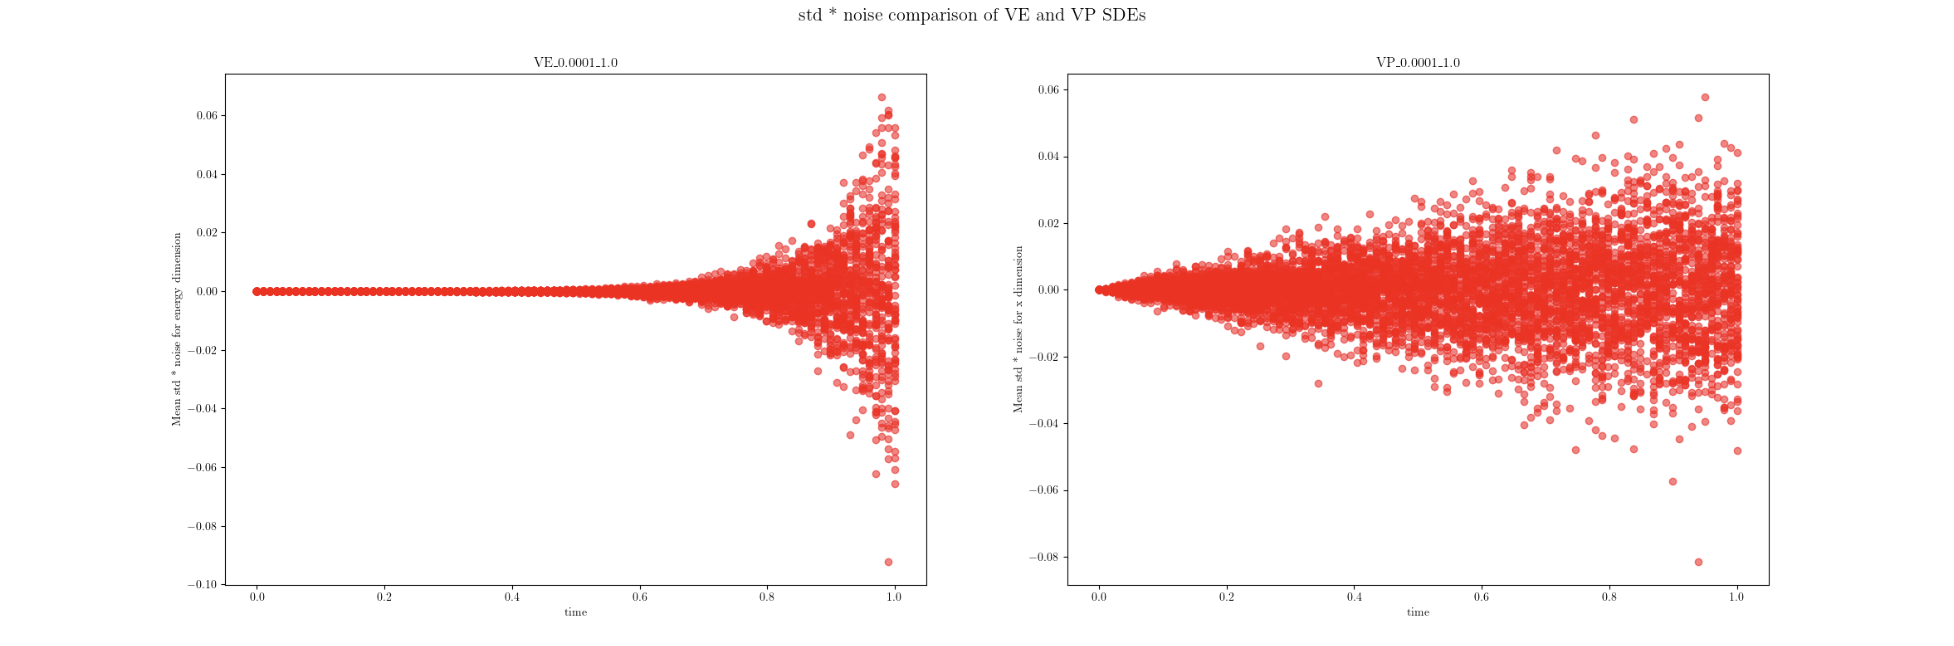
\includegraphics[width=0.8\textwidth,height= 0.35\textwidth]{Figures/sde1.png}
    % Include your loss shape figure here
    \caption{Comparison of VE and VP methods for both $\sigma_{max} = 1, \sigma_{min} = 0.0001$} \label{fig:sde1}
\end{figure}

From Figure \ref{fig:sde1}, it may not be obvious that the value of VE is larger, but later if we see Figure \ref{fig:sde5} and \ref{fig:sde10} when $\sigma_{max} = 5, \sigma_{max} = 10$, we can see that the value of VE is larger than VP.(0.3 vs 0.075) This is consistent with our guess that the VE method will have a better performance than the VP method.

\begin{figure}[h!]
    \centering
    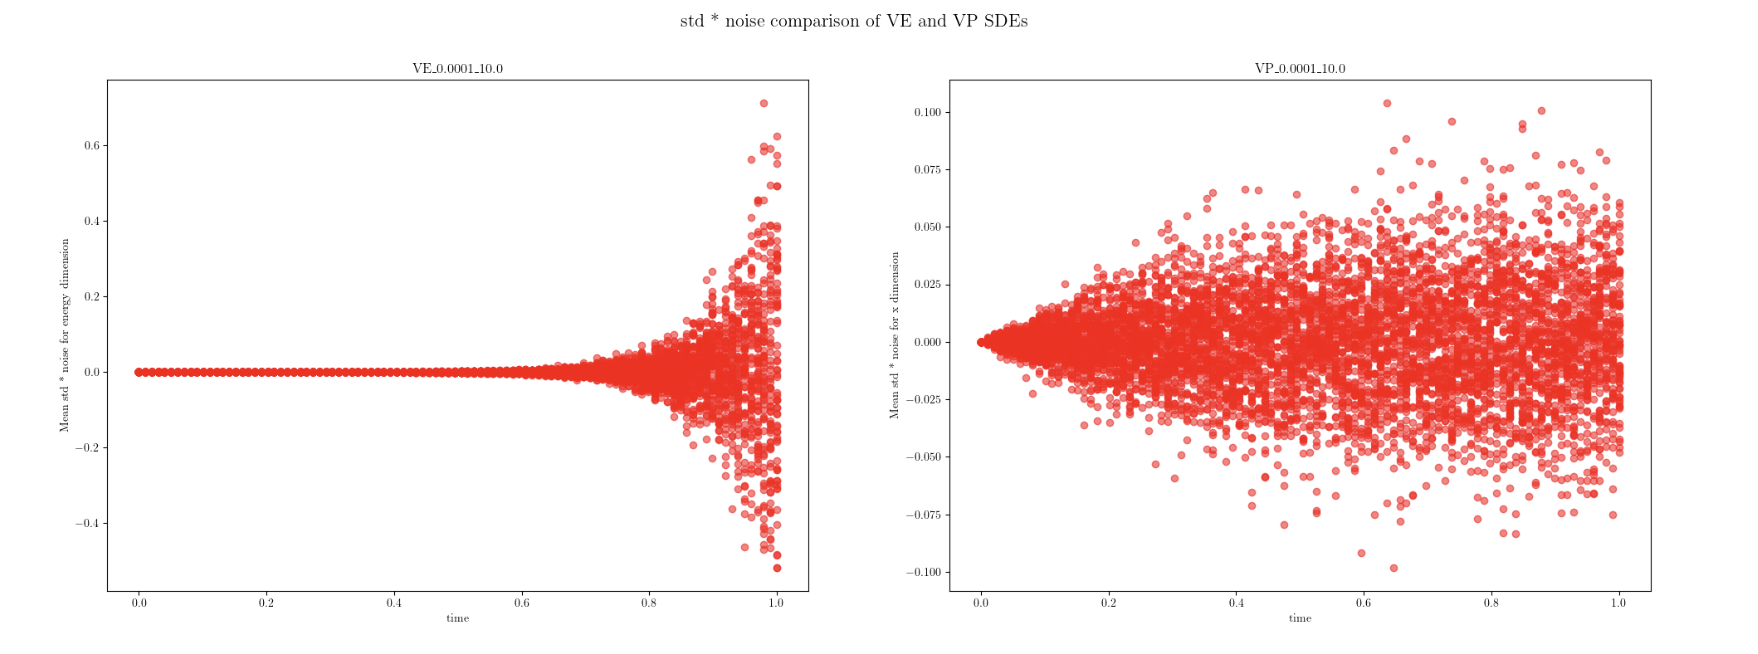
\includegraphics[width=0.8\textwidth,height = 0.35\textwidth]{Figures/sde5.png}
    % Include your loss shape figure here
    \caption{Comparison of VE and VP methods for both $\sigma_{max} = 5, \sigma_{min} = 0.0001$}\label{fig:sde5}
\end{figure}

\begin{figure}[h!]
    \centering
    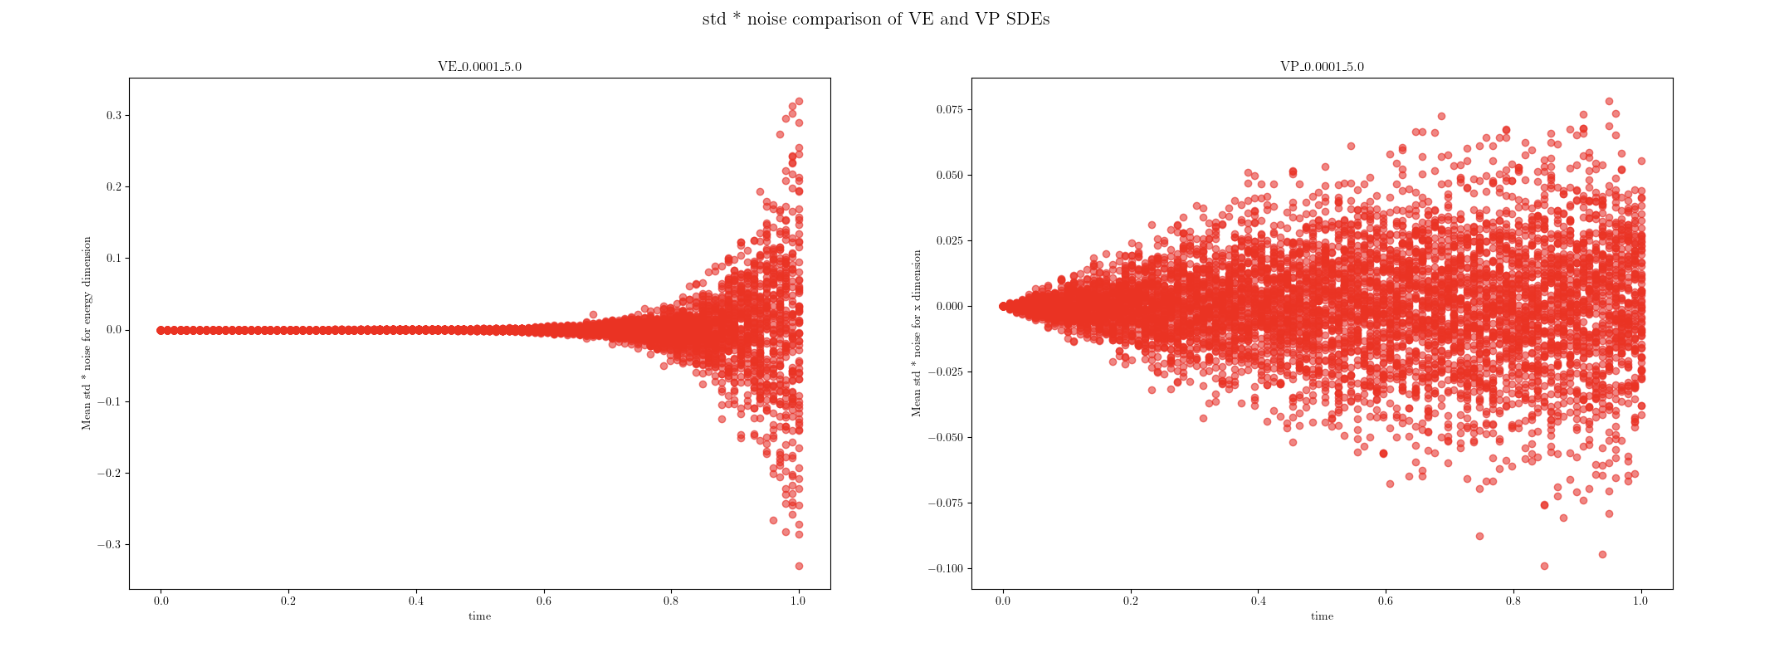
\includegraphics[width=0.8\textwidth, height = 0.35\textwidth]{Figures/sde10.png}
    % Include your loss shape figure here
    \caption{Comparison of VE and VP methods for both $\sigma_{max} = 10, \sigma_{min} = 0.0001$}\label{fig:sde10}
\end{figure}

Next, we can further compare the actual distribution change after adding the noise. We can see that the distribution of the data after adding the noise in the VE method is more close to the random noise than the VP method. This is consistent with our guess that the VE method will have a better performance than the VP method.

\begin{figure}[h!]
    \centering
    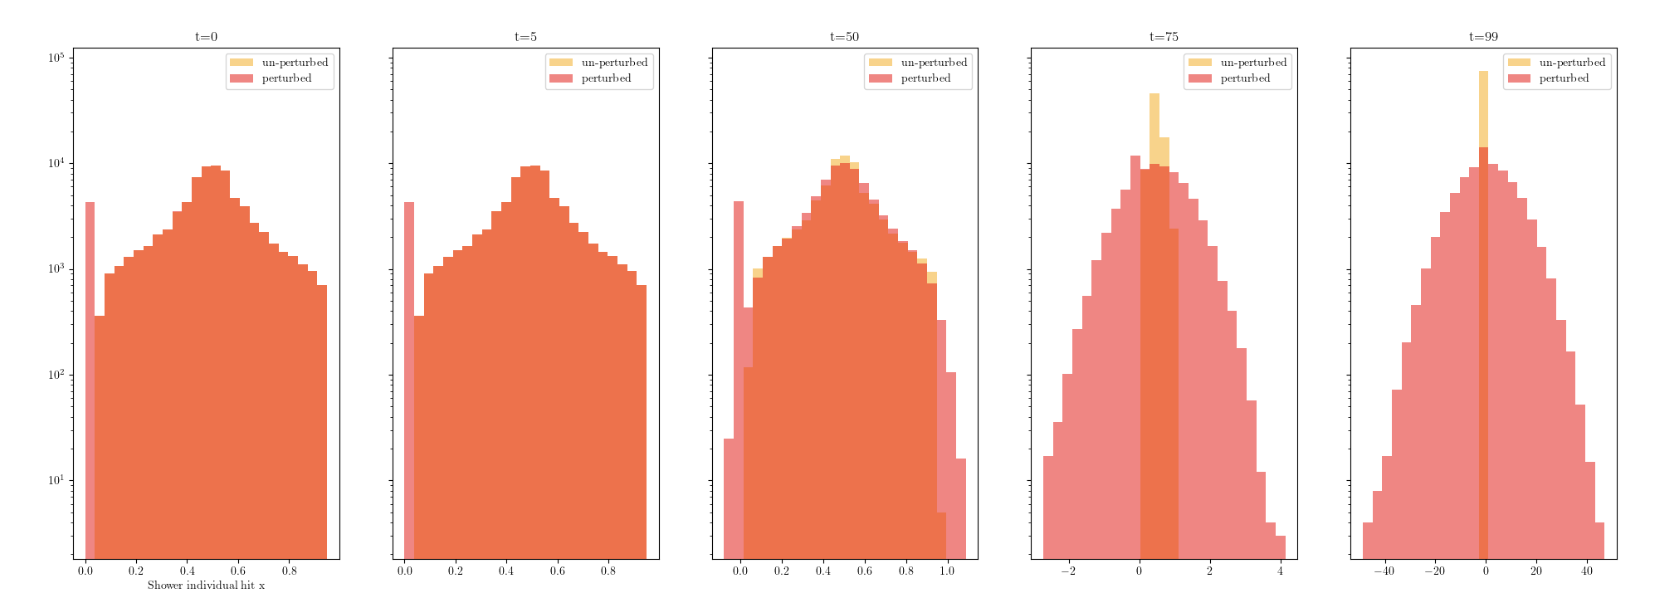
\includegraphics[width=0.8\textwidth]{Figures/VE_5_0.0001.png}
    % Include your loss shape figure here
    \caption{The distribution of the data after adding the noise using VE method.}\label{fig:ve}
\end{figure}

\begin{figure}[h!]
    \centering
    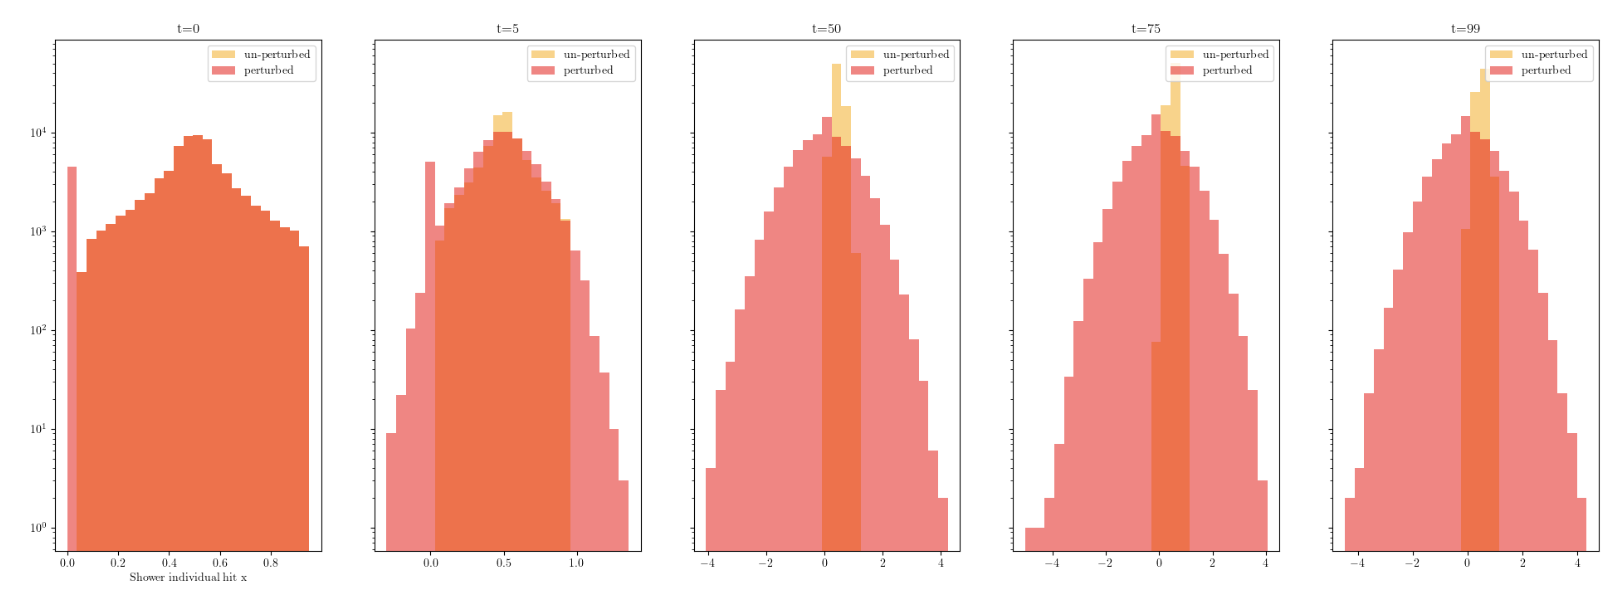
\includegraphics[width=0.8\textwidth]{Figures/VP_5_0.0001.png}
    % Include your loss shape figure here
    \caption{The distribution of the data after adding the noise using VP method.} \label{fig:vp}
\end{figure}

From Figure \ref{fig:ve} and \ref{fig:vp}, we can observe two points. Firstly, the VE method requires more steps to effectively disrupt the original data distribution, allowing the reverse process to provide the model with additional opportunities to capture the true distribution, which is advantageous. Secondly, the distribution of data subjected to noise through the VE method appears closer to random noise than that of the VP method. This observation supports our hypothesis that the VE method is likely to outperform the VP method. 

We also compared the FID scores of models trained with the VE and VP methods. The results showed that the VE method resulted in a lower FID score compared to the VP method. This suggests that the VE method is more effective at pushing the model toward generating random samples that better represent the initial sampling space.

\begin{table}[h!]
    \centering
    % Include your FID score comparison figure here
    \caption{Comparison of FID scores for VE and VP methods.}
\end{table}

In conclusion, the VE method outperformed the VP method in terms of FID score. 
We guess this is because it has more power to push our data to random noise, which is the initial state of sampling space. So our model know how to do the reverse process at the beginning in VE method. For example, if we see the standard deviation of both VE and VP methods, one can find out VE has the steeper slope than VP, which means it has the power to push the data to the random noise.

\section{$\sigma_{max}$ and $\sigma_{min}$ Studies}

Among all fo the parameters, the $\sigma_{max}$ may be the most important one. In the context of diffusion models, the parameters $\sigma_{max}$ and $\sigma_{min}$ play a crucial role in determining the noise levels introduced during the forward and backward processes. These parameters define the range of noise scales, influencing both the quality of the generated samples and the training stability of the model. This section explores the impact of $\sigma_{max}$ and $\sigma_{min}$ on model performance and provides insights into selecting optimal values for these parameters.

\subsection{The Role of $\sigma_{max}$ and $\sigma_{min}$}

The parameter $\sigma_{min}$ represents the minimum noise level in the forward process and also used as the step size of $\sigma$ series. In this case as you can imagine, $\sigma_{min}$ is typically set close to zero. However, based on our abservation, $\sigma_{min}$ won't actually affect too mcuh on the performance of our model. Conversely, $\sigma_{max}$ deos. It defines the maximum noise level and is set high enough to approximate a standard normal distribution. And it also determines the power to change our data distribution during the training. These noise levels influence the progression of the diffusion process, as the model learns to reverse the added noise during training.

Larger $\sigma_{max}$ ensures sufficient diversity in the data during the forward process, helping the model generalize better. Yet, if $\sigma_{max}$ is too large, it can result in excessively noisy samples, making it challenging for the model to learn the reverse process effectively.

\begin{figure}[ht]
    \centering
    % Include your figure here
    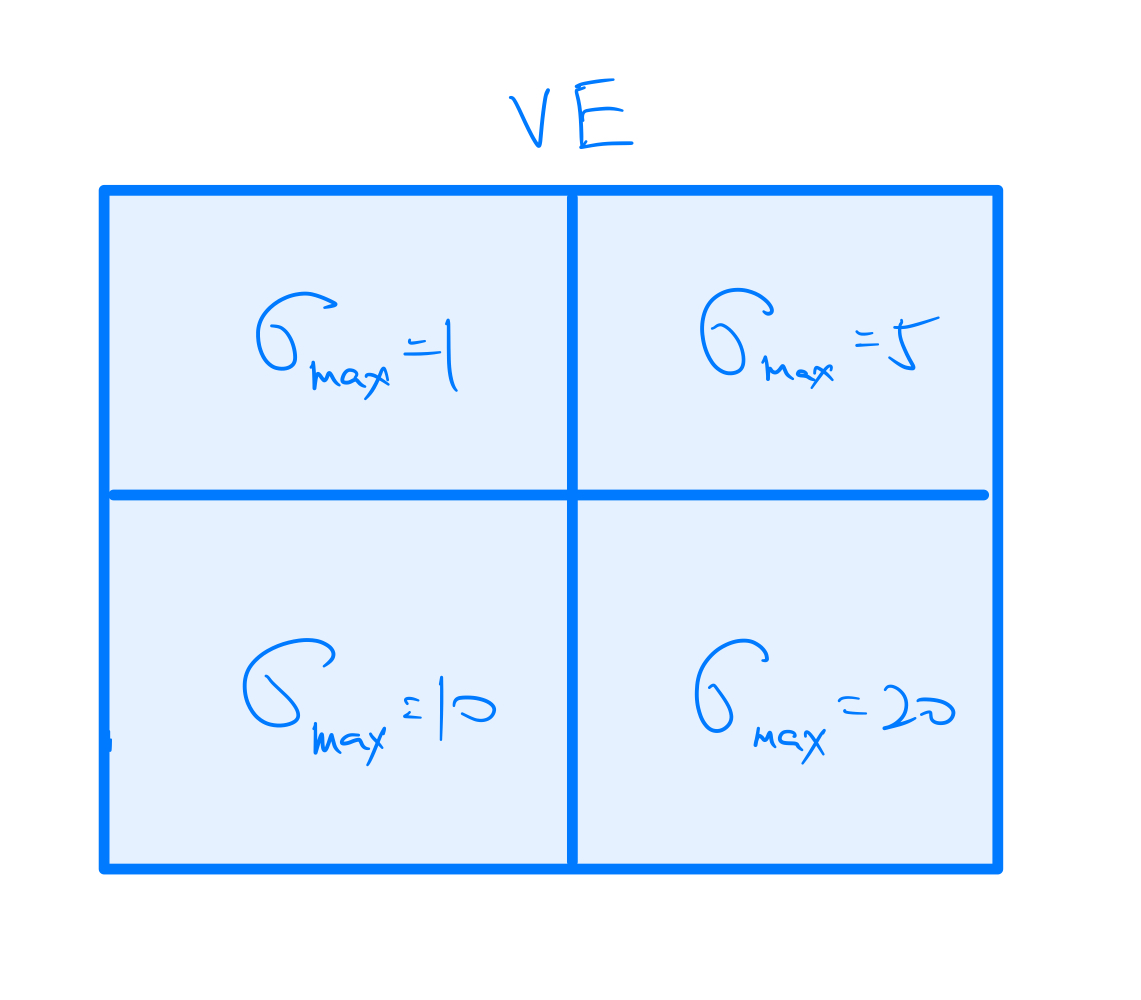
\includegraphics[width=0.8\textwidth]{Figures/VE_sigma_max.jpeg}
    \caption{The result of different $\sigma_{max}$ and $\sigma_{min}$ in VE.} \label{fig:sigma}
\end{figure}

\begin{figure}
    \centering
    % Include your figure here
    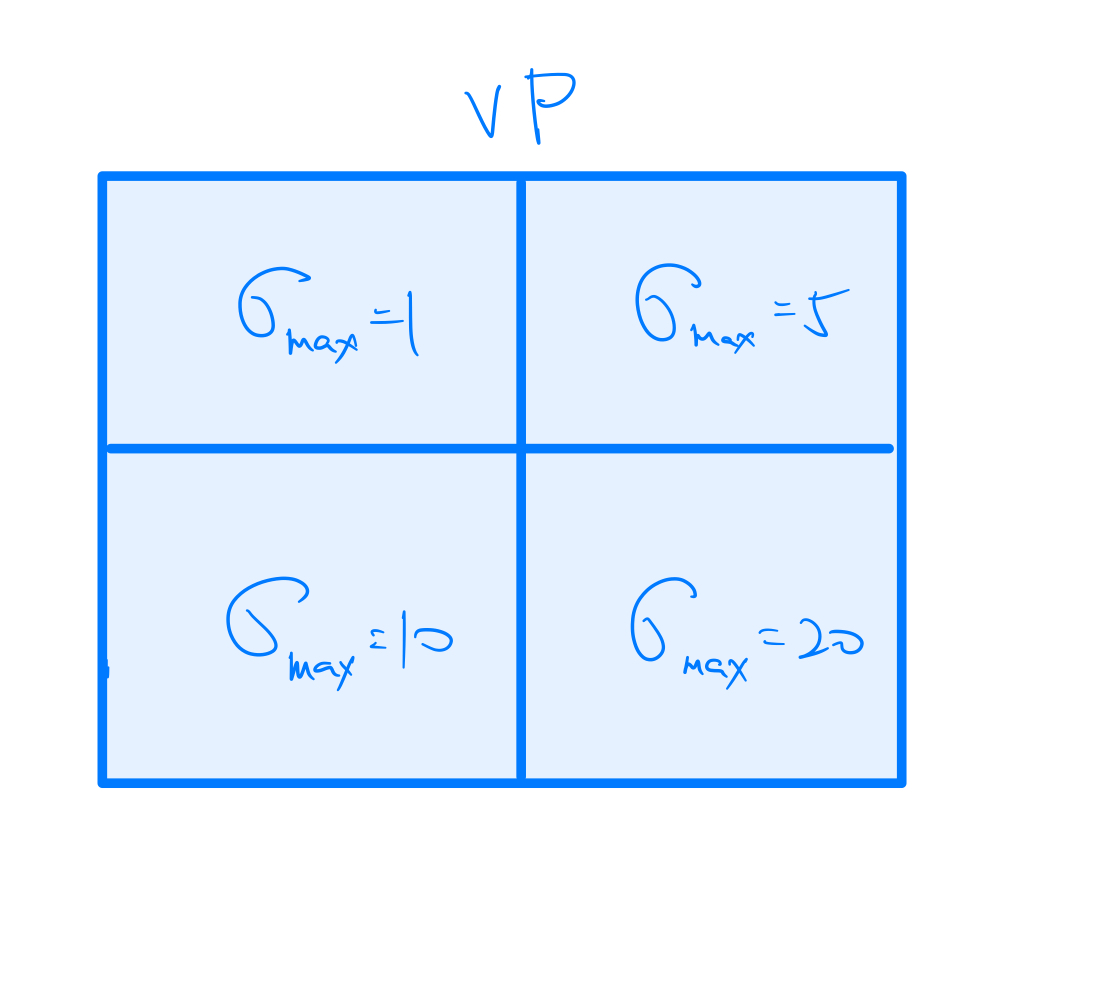
\includegraphics[width=0.8\textwidth]{Figures/VP_sigma_max.jpeg}
    \caption{The result of different $\sigma_{max}$ and $\sigma_{min}$ in VP.} \label{fig:sigma}
\end{figure}

And we can further check the sweep

\begin{figure}[ht]
    \centering
    % Include your figure here
    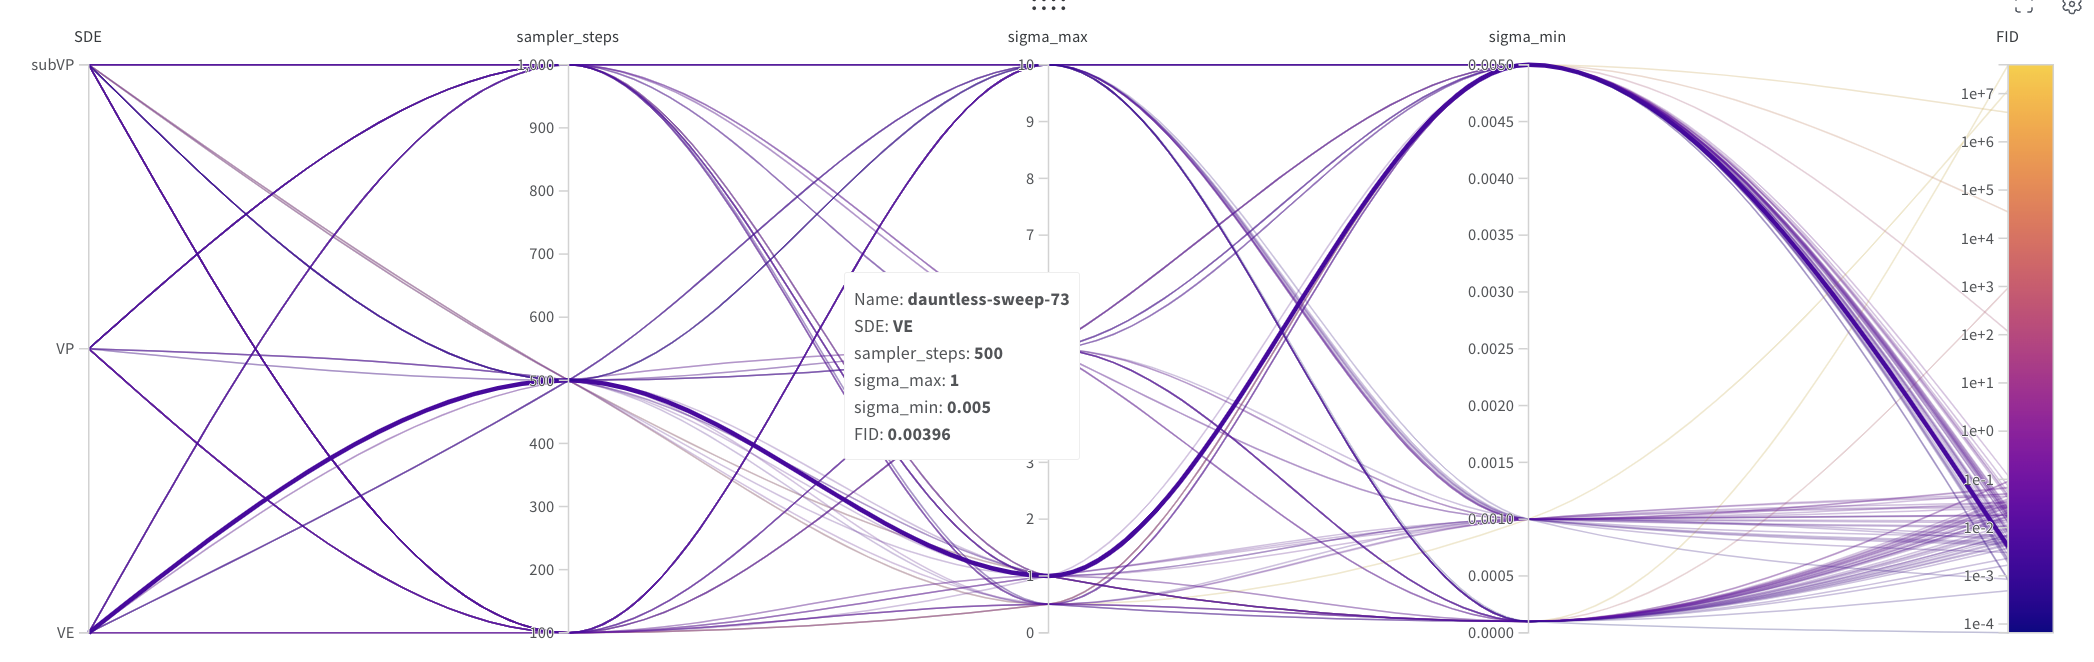
\includegraphics[width=0.8\textwidth]{Figures/sde_sweep.png}
    \caption{The result of different $\sigma_{max}$ and $\sigma_{min}$ in VE.}
\end{figure}

\begin{figure}
    \centering
    % Include your figure here
    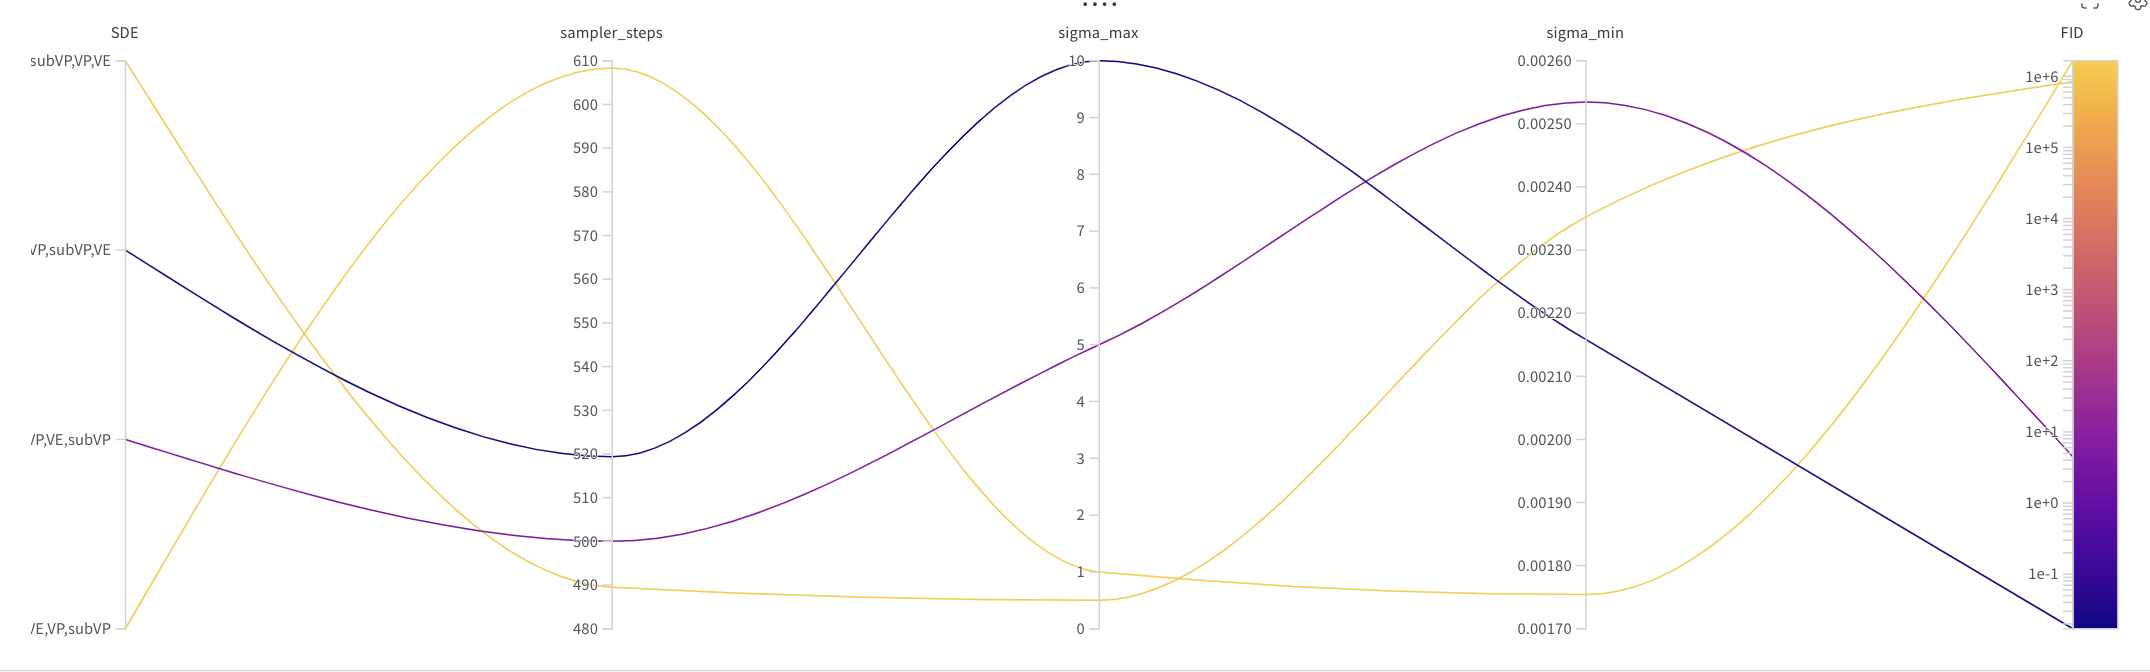
\includegraphics[width=0.8\textwidth]{Figures/sde_sweep_sigmamax.png}
    \caption{}
\end{figure}

\subsection{Conclusions}

As shown in the results, the choice of $\sigma_{max}$ and $\sigma_{min}$ significantly impacts the performance of the model. Larger $\sigma_{max}$ values can improve the diversity of the data and enhance the model's generalization ability. However, setting $\sigma_{max}$ too high can lead to noisy samples and hinder the model's learning process. On the other hand, $\sigma_{min}$ has a less pronounced effect on model performance, as it primarily serves as the step size for the noise levels. And based on our data scale, we choose $\sigma_{min}$ to be 0.0003, and $\sigma_{max}$ to be 5.0 in VE.

\section{Overall Parameter Sweeping}
Besides, the parameters mentioned above there are also a lot of other parameters that can affect the performance of the model or the memory allocation. Thus, we conducted a parameter sweeping study using \texttt{wandb}. We experimented with various learning rates, batch sizes, and hidden dimensions. Our findings indicated that the best-performing parameter configuration was:
\begin{itemize}
    \item Learning rate: $0.0003$
    \item Batch size: $128$
    \item Embedding dimension: $96$
    \item Hidden dimension: $96$
    \item Number of Attention Heads: $8$
    \item Number of Encoder Blocks : $16$
    \item Dropout rate: $0.2$
    \item Sampler Step: $100$
    \item Correction Step: $25$
    \item SDE : VE
    \item Sigma Max: $5.0$
    \item Sigma Min: $0.0003$
\end{itemize}

\begin{figure}[h!]
    \centering
    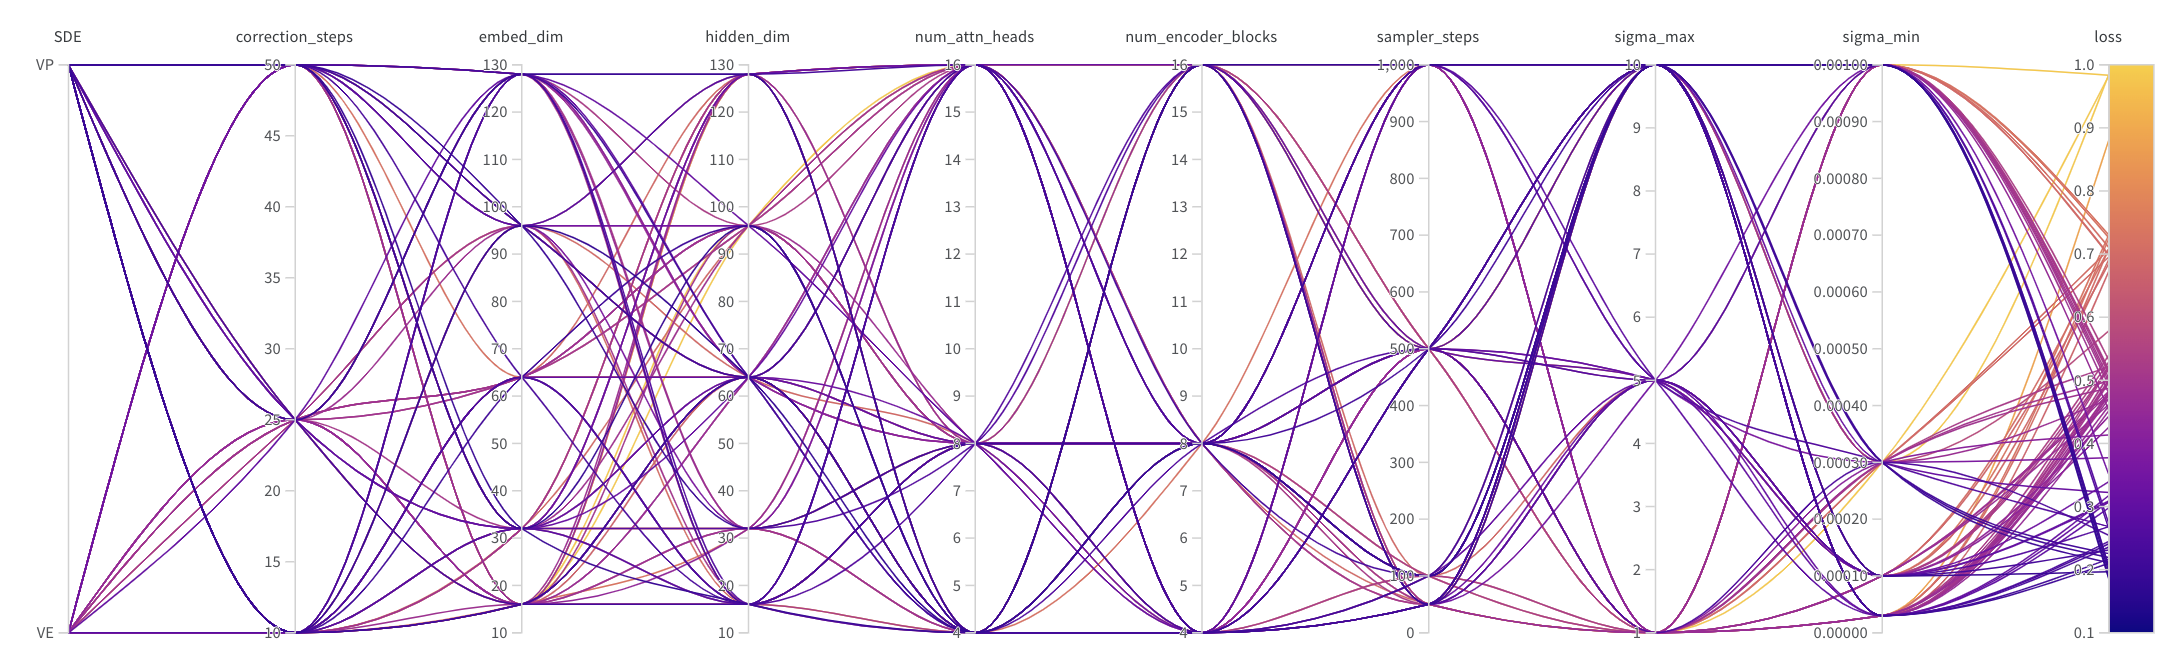
\includegraphics[width=0.8\textwidth]{Figures/other_sweep.png}
    % Include your parameter sweeping study figure here
    \caption{Visualization of parameter sweeping results.}
\end{figure}

\begin{figure}[h!]
    \centering
    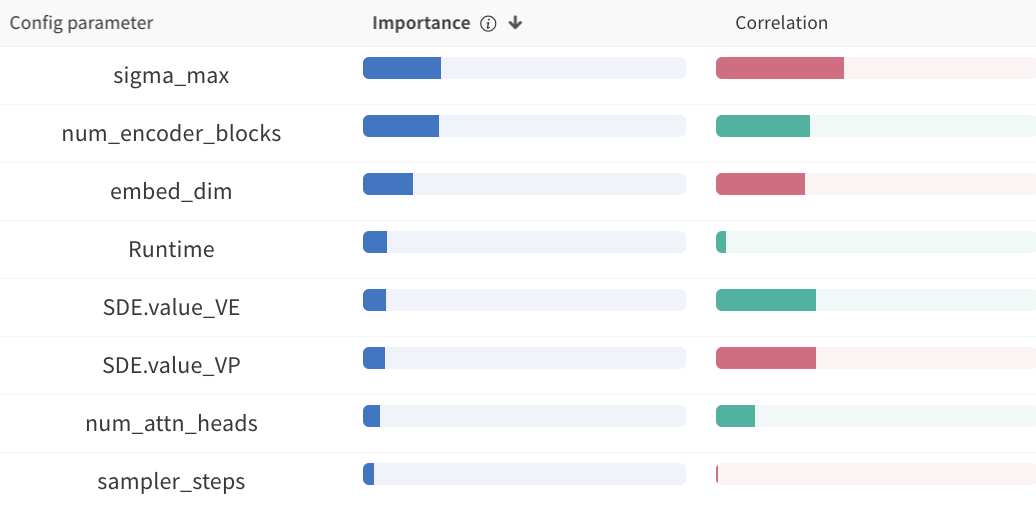
\includegraphics[width=0.8\textwidth]{Figures/sde_importance.png}
    % Include your figure here
    \caption{The result of energy deposit of single bucket data and all bucket data.}
\end{figure}


\section{Centralization}
After visualizing 2D or 3D plots revealed that the model failed to capture the relationship between energy and radius. A key observation was that the model could not learn that higher energy values should be concentrated near the center (smaller radii). Consequently, while the 1D plots were satisfactory, the generated samples lacked proper centralization.

To address this, we first tried to transform our data into spherical coordinate and introduce a correlation term between energy and theta in the loss function to try to suppress relation between energy and theta, hoping our model can thus learn more about the relation between energy and radius. 

The new loss function is defined as:
\begin{equation}
    L = L_{\text{MSE}} + \lambda L_{\text{cor}},
\end{equation}
where $L_{\text{MSE}}$ is the mean squared error loss, $L_{\text{cor}}$ is the correlation loss, and $\lambda$ is a weighting factor for the correlation loss. The correlation loss is defined as:
\begin{equation}
    L_{\text{cor}} = \frac{1}{N} \sum_{i=1}^{N} (x_i - \bar{x})(y_i - \bar{y}),
\end{equation}
where $x$ and $y$ are the variables of interest, and $\bar{x}$ and $\bar{y}$ are their respective means.

The reason why we don't apply the correlation term between energy and radius is that the relation between them is by experienced, although everyone would expect the result, it's not solid, we don't want to bias our model, or you can say we don't want to tell the answer of the relation to our model. 

However, although the correlation term was added to the loss function and it indeed suppressed the relation between energy and theta, the centralization of the generated samples did not improve significantly. This suggests that the correlation term alone is not sufficient to address the centralization issue.

\begin{figure}[h!]
    \centering
    % Include any relevant results or visualizations here
    \caption{The Picture after adding the correlation term.}
\end{figure}

After that, one time when we tried to use QuantileTransformer to preprocess the data, we found that the centralization of the data is improved. This is because the QuantileTransformer can transform the data to follow a uniform or a normal distribution. This can help the model to learn the data better, especailly the x,y distribution. This also makes it is able to learn the relation between energy and radius better.

The result compared to the original one is shown below:

\begin{figure}[h!]
    \centering
    % Include any relevant results or visualizations here
    \caption{The Comparison Picture after using QuantileTransformer.}
\end{figure}

\section{Conditioning Issue}
\subsection{incident energy}
With the optimal settings, our model was able to generate the basic shapes of both the energy and spatial distributions. However, the model often produced an excessive number of hits (\texttt{nhits}) at higher energy levels, leading to overestimation. This issue was not observed when training on single-bucket data, indicating that the model struggles to differentiate between data from different buckets. This suggests that our conditional variables are not functioning effectively. As you can see the result of energy deposit of single bucket data and all bucket data, the model can generate the data well in single bucket data, but it failed to generate the data well in all bucket data. This is because the model can't learn the condition well.

\begin{figure}[ht]
    \centering
    % Include your figure here
    \caption{The result of energy deposit of single bucket data and all bucket data.}
\end{figure}

To address this issue, we first need to make sure if our conditional variables aren't really working. So we tried to add the incident energy as the conditional variables and not. The result is shown below:

\begin{figure}[ht]
    \centering
    % Include your figure here
    \caption{The result of energy deposit with and without incident energy as conditional variables.}
\end{figure}

They are basically the same, indicating that the conditional variables are not working. Next, we also tried to concatenate the incident energy with the input data instead of adding them and the result is shown below:

\begin{figure}[ht]
    \centering
    % Include your figure here
    \caption{The result of energy deposit with incident energy concatenated with the input data.}
\end{figure}

As you can see, the result is totally a disaster. To be honest, we still don't know why this happened. 

Next, we move to even more complex conditional variables. We have tried class token. The result is shown in Figure ~\ref{fig:energy_deposit}:

\begin{figure}[ht]
    \centering
    % Include your figure here
    \caption{The result of energy deposit with class token.}\label{fig:energy_deposit}
\end{figure}

\subsection{Time}

We also attempted to incorporate time as a conditional variable in our model. However, the results differ from those observed with incident energy. Even without explicitly using time as a condition, the output layer implicitly incorporates its effect by dividing by the standard deviation of the stochastic differential equation (SDE), which is time-dependent. Despite this, the inclusion of time as a conditional variable does not appear to enhance the model's performance.

The plot of loss versus time reveals consistent behavior across epochs, showing that the shape of this plot remains virtually unchanged. Notably, the loss value at $t = 0$ is almost identical to the initial loss, indicating that the time condition fails to improve the model's capacity to learn the data effectively.

Time close to $t = 0$ represents the critical phase where the model transitions toward generating real data, whereas near $t = 1$, the model predominantly learns the structure of Gaussian noise. This suggests that the model's learning mechanism may inherently prioritize earlier time steps, making additional time conditioning redundant or ineffective.

\begin{figure}[ht]
    \centering
    % Include your figure here
    \caption{The loss vs time plot.}
\end{figure}





